% Chapter Template

\chapter{Methodology} % Main chapter title
The following chapter will describe the problem that investigated in this work, the model adjustments and definitions,
the methods and the tools used to do so.

\label{chap:methodology} % Change X to a consecutive number; for referencing this chapter elsewhere, use \ref{ChapterX}

%----------------------------------------------------------------------------------------
%	SECTION 1
%----------------------------------------------------------------------------------------

\section{Problem definition}
\label{sec:problemDef}
%The goal of modeling is always to invent a model that is capable of correctly reproducing past and reliably predicting 
%future events. The latter is often very difficult, since it is necessary to correctly understand the dynamics of a
%complex system and then implement these dynamics in the form of a program, algorithm or method.\newline

%\par
The previous work of \cite{Rastogi} investigated the SEIRD model on a 2d-grid of Germany. In his work he simulated
all five groups of the SEIRD model for seven cities in Germany. This proved that the model itself is functional and
in principle capable of reproducing and predicting \textcolor{red}{(?)} the dynamic of the COVID-19 epidemic. This % note
is where this work continued.\newline

\par
The goal of this work was to better understand the performance of the model in a smaller scale environment and to improve
the quality of the results. Hesse (Germany) and its regions where chosen as a template for a new 2d-grid. To minimize the
propagation of error throughout the SEIRD groups, we decided to focus on optimizing the equation variables
\textcolor{red}{(add reference to equations)} % note
of each group successively. In this work we focused on the Susceptible (S) group and tried to reproduce/predict real world
data and upcoming trends. Additionally we focused on evaluating the sensitivity of the S group to the two variables
$\alpha$ and $q$.

%-----------------------------------
%	SECTION 2
%-----------------------------------
\section{Model adjustment and data acquisition}


%-----------------------------------
%	SUBSECTION 1
%-----------------------------------
\subsection{Data acquisition}
\label{sec:datacoll}
In order to run the SEIRD model, it was necessary to gather real world data for as many of the five groups as possible.
The source for this data was the Github project \cite{Gehrcke}, which provided both the number of COVID-19 infections,
as well as the number of COVID-19 related deaths per region in Germany. The repository provides data based on the case/death
numbers published by the RKI (Robert Koch Institute) and the Risklayer GmbH. In this work the data based on the RKI publications
was used. The data format were cumulative case/death numbers per region per day.\newline

\par
The hospitalization rate of confirmed COVID-19 infected individuals, the average time till symptom onset, the average time till
hospitalization and the lethality rate case of an infection was taken from RKI publications \cite{RKIcov}. At the time of acquisition, these
numbers were only estimations based on the literature of the current date.\newline

\par
The population of each region in Hesse was taken from the website ``statistic.hessen.de''. The data was sourced from \cite{HessePop}
in the category ``Bef\"olkerung in Hessen 2017 bis 2020 nach Verwaltungsbezirk in Monaten''. The size of each region in Hesse
was taken from \cite{HesseSize}.

%-----------------------------------
%	SUBSECTION 2
%-----------------------------------
\subsection{SEIRD model adjustments}
\label{sec:SEIRDredef}
In order to reach the goals described in \hyperref[sec:problemDef]{section \ref*{sec:problemDef}}, we decided to alter
the definitions of the Exposed (E) and Infected (I) groups. Furthermore we decided to set the variable
$\kappa$ to 1, effectively removing the option of exposed individuals to recover without developing symptoms. These
changes were done for two major reasons:\newline

\par
First, data availability proved to be an issue. The problem being, that the number of infected in the
collected data set only includes individuals that were tested positive with a polymerase chain reaction (PCR) test\cite{??}. However,
these tests are usually conducted, if an individual is experiencing symptoms of sickness\cite{??}. This means, that individuals, that do
not experience symptoms are (for the most part) not represented in the collected data. In addition, it is difficult to estimate
the ratio between infected individuals that experience symptoms and individuals that do not experience symptoms. This makes it
even harder establish realistic assumptions, on which bases the original data could be modified to account for this phenomenon.\newline

\par
The second reason for these changes is a better representation of the actual disease history of COVID-19. Generally individuals that
are infected with COVID-19, are contagious to others before they develop symptoms. While sick individuals can infect others many
days after symptom onset, about halve of all transmissions are pre-symptomatic (the infection event occurs before symptom onset)
\cite{casey2021presymptomatic} and that symptom onset generally reduces transmission rates due to isolation measures\cite{RKIcov}.

\par
Based on this findings, we did not allow for direct recovery from the model and redefined redefined the E and I groups as such: 
\begin{enumerate}[label=$\bullet$]
	\item \B{Exposed (E)}: Group of individuals that are infected with the virus and will develop symptoms in the upcoming
		days. Individuals are contagious during this time and contribute to infections of susceptibles.
	\item \B{Infected (I)}: Group of individuals that has experienced symptoms. Individuals are mostly not contagious anymore
		and isolate themself/are isolated until recovery or death.
\end{enumerate}

\textcolor{red}{(might need better reasoning)} %note

%----------------------------------------------------------------------------------------
%	SECTION 2
%----------------------------------------------------------------------------------------

\section{Experimental setup and pre-simulation work}
The following section will describe the assumptions made based on the previous explanations, the generation of a suitable data set and
the pre-processing of the newly created data.


%-----------------------------------
%	SUBSECTION 1
%-----------------------------------
\subsection{Assumptions}
Based on the information we gathered, as described in \hyperref[sec:SERIDredef]{section \ref*{sec:SEIRDredef}}, we made a set of assumptions
in order to derive our experimental data from the raw data. These assumptions are as follows:

\begin{enumerate}
	\item The average time for an infected individual to develop symptoms is 6 days.
	\item After symptom development, an individual begins self isolation and does not contribute to new infections.
	\item The average time for a symptomatic individual to lose most of its contagiousness is about 10 days. This was defined as
		transition to the recovered (R) state.
	\item The average time between symptom onset and death was about 11 days during the first infection wave in Germany. This was
		defined as transition to the diseased (D) state.
	\item Based on 3. and 4. we estimated a transition time from the exposed (E) state to either R or D of 10 days. Using the
		average of 10.5 days was not possible, since only one data point per day was available.
\end{enumerate}


%-----------------------------------
%	SUBSECTION 2
%-----------------------------------
\subsection{Data pre-processing}
Since the raw data was cumulative, the number of individuals in each group at time point $t$ were defined as follows:

\begin{align}
	S(t) &= N - i(t+6)\\
	E(t) &= i(t+5) - i(t)\\
	I(t) &= i(t) - i(t-10)\\
	R(t) &= i(t-10) - d(t)\\
	D(t) &= d(t)
\end{align}

\par
Where $N$ represents the total number of individuals living in a specific region of Hesse at the beginning of the pandemic, $i(t)$
represents the cumulative number of infected individuals at time $t$ and $d(t)$ represents the cumulative number of deceased
individuals at time $t$. These calculations were done for each region, time point and group.\newline

\par
We chose to simulate the time frame between 01\I{st} September 2020 and the 15{th} of November 2020 (a time frame of 76 days). These
data points were chosen, since no
\textcolor{red}{(check to be sure)} %note
significant policy changes regarding protective measures against COVID-19 infections (mask mandates, isolation periods, store closures) 
were made during this time in Germany. Additionally this time frame was before other COVID-19 variants were first observed in
Germany\cite{??}. It can therefore be assumed, that only the original CODIV-19 strain from Wuhan was contributing to infections.
This minimizes the risk of phenomena influencing the simulation reluslts, that are not accounted for in the model.\textcolor{red}{(rewrite sentence? kinda shit...)}\newline

\par
Each group was calculated for each day in each region. For the first day of simulation (day 0), the percentage of each group at that
point in time was calculated. These values were used as the starting point for our simulations.


%-----------------------------------
%	SUBSECTION 2
%-----------------------------------
\subsection{Generation of Hesse 2d-grid}
For the simulation, a 2d-grid of Hesse was created using the program ProMesh4. The grid was manually drawn and consisted
of 1075 vertices and 3049 edges, from which 1975 faces (triangular volumes) were constructed. The grid can be refined
to 4136 vertices (accompanied also by an increasing number of edges and faces), however during this work only the grid
with 1075 vertices was used for simulations. The grid itself was divided into 26 regions, representing the 26 autonomous
regions of Hesse. A visual representation of the grid with and without wire frame and an exemplary image of the original geogrphay
of Hesse are shown in \hyperref[fig:2d-grid]{Figure \ref*{fig:2d-grid}}.

\begin{figure}
	\begin{center}
		\begin{subfigure}[b]{0.3\textwidth}
			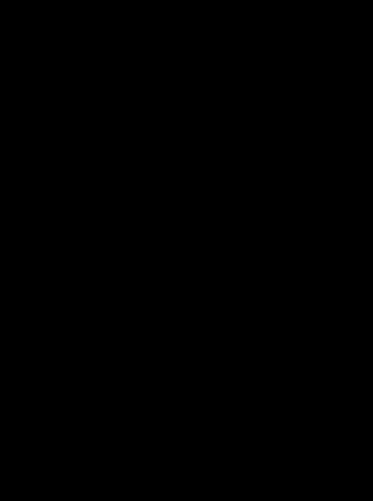
\includegraphics[width=\textwidth]{./figures/2d_grid_test.png}
		\end{subfigure}
		% ---------------------
		\begin{subfigure}[b]{0.3\textwidth}
			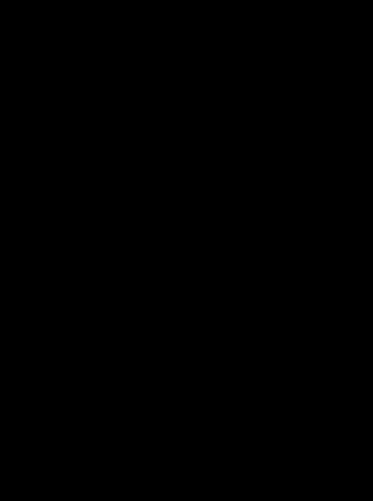
\includegraphics[width=\textwidth]{./figures/2d_grid_test.png}
		\end{subfigure}
		% ---------------------
		\begin{subfigure}[b]{0.3\textwidth}
			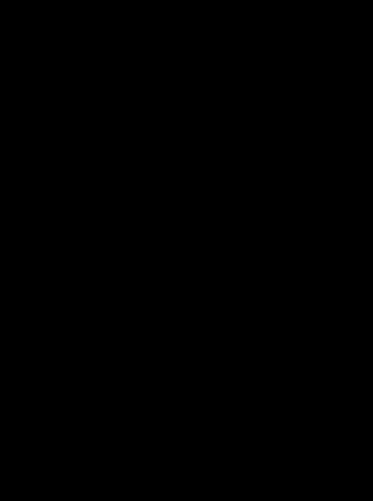
\includegraphics[width=\textwidth]{./figures/2d_grid_test.png}
		\end{subfigure}
	\end{center}
	\caption{caption of the 2d-grid}
	\label{fig:2d-grid}
\end{figure}

The geometry and properties of the grid (also called mesh in the context of computational simulation) make it unstructured.
That means, that vertices can be positioned and connected arbitrarily. This method provides more flexibility then 

\textcolor{red}{add finite volume explanation}

%----------------------------------------------------------------------------------------
%	SECTION 3
%----------------------------------------------------------------------------------------

\section{SEIRD simulation}

-simulation itself without optimization

\subsection{ODE}


\subsection{LIMEX scheme}


\subsection{Solvers}

%----------------------------------------------------------------------------------------
%	SECTION 3
%----------------------------------------------------------------------------------------

\section{Data post-processing and variable optimization}

%-----------------------------------
%	SUBSECTION 1
%-----------------------------------
\subsection{Output-grid association}
- results associated to grid vertices via new program

%-----------------------------------
%	SUBSECTION 2
%-----------------------------------
\subsection{Loss function}
- loss function\\

%-----------------------------------
%	SUBSECTION 3
%-----------------------------------
\subsection{Variable optimization via ConstrainedOptimization}
- simulation methods Gauss/PSO
